\chapter{基于强化学习的对抗性恶意软件生成方法研究方案 Research Solution for Adversarial Malware Generation Technology Based on Reinforcement Learning}

本章将具体地介绍本文提出的对抗样本生成方法的详细设计过程和实现原理,主要包括扰动方法的构建,奖励函数策略的设计,模型的具体结构。

This chapter will specifically introduce the detailed design process and implementation principles of the adversarial sample generation method proposed in this research, which mainly includes disturbance methods' construction, the reward function strategies' design, and the model's specific structure.

\section{多维度扰动方法的构建 Multidimensional Disturbance Methods' Construction}

本文利用lief库、IDA pro对二进制可执行样本进行批量处理。LIEF(Library to Instrument Executable Formats)是一个开源的库,用于处理ELF、PE和Mach-O格式的可执行文件。它可以解析和修改二进制文件的头部信息、节区、符号和动态链接。LIEF适用于静态分析、重命名符号、插入代码和文件格式转换等任务。LIEF可以提取二进制可执行文件的结构,以及提供各个结构的操作接口。

This research batch processes binary executable samples using the LIEF library and IDA Pro. LIEF (Library to Instrument Executable Formats) is an open-source library for processing executable files in ELF, PE, and Mach-O formats. It can parse and modify header information, sections, symbols, and dynamic linking in binary files. LIEF is applicable to tasks such as static analysis, symbol renaming, code insertion, and file format conversion. LIEF can extract the structure of binary executable files and provide operation interfaces for various components.

\subsection{结构化扰动方法 Structural Disturbance Methods}

在恶意软件的对抗性样本生成过程中,结构层面的扰动指的是通过修改文件的内部结构来引入变化,这种变化通常不会影响文件的执行逻辑,但能够有效地逃避传统的检测方法。结构层面的扰动包括但不限于文件的节区、导入符号、动态库、以及压缩/解压缩等操作。

In the adversarial malware sample generation process, structural level disturbances refer to introducing changes by modifying a file's internal structure. These changes commonly do not affect the file's execution logic but effectively evade traditional detection methods. Structural level disturbances include operations on sections, imported symbols, dynamic libraries, compression, and decompression, but are not limited to these.

这些扰动主要关注的是通过改变文件结构中的某些元素来达到以下目的:

These disturbances primarily concentrate on achieving the following purposes by altering certain elements in the file structure:

增加文件的不可预测性:通过随机化或改变文件的某些部分,使得检测系统很难依赖固定模式进行识别。

Increasing file unpredictability: By randomizing or changing parts of the file, detection systems hardly identify the file, relying on fixed patterns.

避开静态分析:静态分析工具通常依赖文件的固定结构特征,如节区(Section)、符号表、导入表等。通过扰动这些结构,可以增加检测的难度。

Evading static analysis: Static analysis tools often depend on fixed file structural features, such as sections, symbol tables, and import tables. Disturbing these structures increases detection difficulty.

防止签名匹配:一些恶意软件检测工具依赖于已知恶意样本的特征(如哈希值、节区结构等)进行匹配。通过扰动结构,可以使文件与原始恶意样本在这些特征上产生差异,从而避开检测。

Avoiding signature matching: Some malware detection tools rely on known signatures, such as values, section structures from malicious samples. Disturbing structures creates differences between the file and the original malicious sample in these signatures, enabling evasion.

(1)节区(Section)扰动

(1) Section Disturbance

在ELF(Executable and Linkable Format)文件中,节区是文件的基本构建单元。它们存储了不同类型的数据(如代码、数据、符号等)。通过对节区内容进行扰动,可以修改文件的行为或使其变得更加复杂。常见的节区扰动方式包括:

In ELF files, sections are the fundamental units, storing different types of data, such as code, data, symbols. Disturbing section content can modify file behavior or increase its complexity. Common section perturbation methods include:

节区内容的修改:例如,在现有节区中附加随机数据、将特定节区的数据替换为 benign 数据(如无害的字符串或二进制内容)等。这样可以增加恶意文件的复杂性并避免与已知恶意样本的特征匹配。

Modifying section content: For example, appending random data to existing sections or replacing data in specific sections with benign data like harmless strings or binary content increases malicious files’ complexity and avoids matching known malicious sample signatures.

节区重命名:将节区名称修改为常见的名称或随机名称,使得检测工具无法轻易识别文件中的关键节区,如 .text 节区,通常包含程序代码。

Renaming sections: Changing section names to common or random names makes it harder for detection tools to identify critical sections, especially the .text section that contains program code.

本文设计的节区扰动如表\ref{tab:4.1}所示。

The section disturbance design in this paper is listed in Table \ref{tab:4.1}.

\begin{table}[htbp]
	\centering
	\caption{节区扰动类型}\label{tab:4.1}
	\begin{tabular*}{\textwidth}{@{\extracolsep{\fill}}ccc}
		\toprule
		扰动 & 简写 & 效果 \\
		\midrule
		section\_append & SA & 向随机选择的节中追加随机数据(可能改变节的内容和熵) \\
		add\_section\_benign\_data & ASBD & 从 benign 文件中提取整个节,并添加到目标 ELF 中 \\
		add\_section\_strings & ASS & 生成一个新的节,填充 benign 字符串内容 \\
		section\_rename & SR & 随机重命名一个节,使用常见节名列表中的名称 \\
		\bottomrule
	\end{tabular*}
\end{table}

(2)导入符号和库扰动

ELF文件中的导入符号表(dynamic symbol table)包含了程序运行时需要链接的外部函数或库。通过扰动这些符号,可以使恶意软件的行为更加不可预测。例如:

添加恶意符号:将恶意的动态符号(如恶意函数名)添加到文件中,或者通过与良性文件进行符号混合,增加文件的复杂性。

修改库依赖:修改ELF文件所依赖的动态库,使其依赖于一个不存在或不常见的库,从而打乱传统的静态分析过程。

本文设计的导入符号和库扰动如表\ref{tab:4.2}所示。

\begin{table}[htbp]
	\centering
	\caption{导入符号和库扰动}\label{tab:4.2}
	\begin{tabular*}{\textwidth}{@{\extracolsep{\fill}}ccc}
		\toprule
		扰动方法 & 简写 & 效果 \\
		\midrule
		add\_imports & AI & 从 benign ELF 文件中添加一个动态符号到目标 ELF 中(如函数导入) \\
		add\_library & AL & 从 benign ELF 文件中添加一个共享库和其导入函数 \\
		\bottomrule
	\end{tabular*}
\end{table}


(3)随机数据附加(Overlay)

Overlay技术通过在文件末尾添加随机数据(通常是无害数据或伪装数据),可以在不改变文件执行流程的情况下修改文件的大小和结构。这种技术常用于恶意软件中以绕过基于签名的检测。常见的技术包括:

追加随机字节:将随机的字节序列附加到ELF文件的末尾。此操作不会影响文件的执行逻辑,但可能会改变文件的哈希值,使其避开传统的哈希匹配检测。

追加无害二进制文件内容:从已知的良性文件中提取节区或二进制内容,插入到恶意文件中,以增加文件的复杂度并扰乱静态分析工具的检测。

\begin{table}[htbp]
	\centering
	\caption{随机数据附加类型}\label{tab:4.3}
	\begin{tabular*}{\textwidth}{@{\extracolsep{\fill}}ccc}
		\toprule
		扰动方法 & 简写 & 效果 \\
		\midrule
		overlay\_append & OA & 在二进制文件的末尾附加随机内容 \\
		append\_benign\_data\_overlay & ABDO & 追加来自 benign ELF 文件 .text 段的内容 \\
		append\_benign\_binary\_overlay & ABBO & 直接追加整个 benign ELF 文件内容 \\
		add\_strings\_to\_overlay & ASTO & 追加来自 benign 字符串文件的内容(UTF-8 编码) \\
		\bottomrule
	\end{tabular*}
\end{table}

(4)压缩与解压缩(UPX打包与解包)

压缩恶意文件是另一种常见的扰动技术。通过使用UPX等压缩工具对ELF文件进行压缩,可以隐藏文件的原始结构,并使文件在未经解压时不可执行。这种方法主要有以下特点:

压缩:压缩文件可以改变文件的内部结构,使其看起来与原始文件完全不同,从而避开基于特征的检测。

解压缩:压缩的ELF文件在运行时会被解压缩回原始状态,因此需要额外的解压步骤。通过这种方式,恶意软件的行为和文件结构可以被“隐藏”在压缩层后面,增加了反向工程和静态分析的难度。

\begin{table}[htbp]
	\centering
	\caption{压缩加壳类型}\label{tab:4.4}
	\begin{tabular*}{0.9\textwidth}{@{\extracolsep{\fill}}ccc}
		\toprule
		扰动方法 & 简写 & 效果 \\
		\midrule
		upx\_pack & UP & 使用 upx 对 ELF 文件进行压缩 \\
		upx\_unpack & UUP & 使用 upx -d 解压已压缩的 ELF 文件 \\
		\bottomrule
	\end{tabular*}
\end{table}

(5)Go语言的go-bindata工具包装ELF文件

go-bindata是一个Go工具,旨在将二进制文件(如ELF文件、图片、音频文件等)转化为Go源代码中的字节数组。在恶意软件分析领域,通过将ELF文件嵌入到Go程序中,可以有效隐藏ELF文件的实际内容,并增加静态分析和反向工程的难度。具体而言,go\_bindata\_wrapper方法通过将ELF文件转换为Go代码,实现在Go程序中隐藏ELF文件的功能。这种方式使得恶意文件能够避开常规的静态检测和签名匹配工具。

go-bindata工具的作用:go-bindata工具将任何二进制文件(如ELF文件)嵌入到Go源代码中,并生成一个包含文件内容的Go文件。在程序运行时,生成的Go文件将包含文件的字节数组,这些字节数据可以被Go程序读取,并用于恢复原始文件内容。此方法使得ELF文件内容隐藏在Go源代码中,从而增加了恶意软件在反向工程过程中的隐蔽性。

通过go-bindata工具将ELF文件转换为Go源代码,并生成一个Go文件,Go文件中包含该ELF文件的字节数据。通过Go编译器将包含ELF文件字节数据的Go代码编译成最终的Go可执行文件。ELF文件在运行时会被读取并恢复,执行原始文件的操作。

通过go-bindata工具,go\_bindata\_wrapper方法为恶意文件提供了一种新的隐蔽方式,将ELF文件嵌入到Go程序中,从而有效地规避静态分析工具和签名匹配的检测。

(6)节头表修改

节头表扰动旨在通过修改二进制文件中的特定元数据或表头信息,从而改变其表象特征,扰乱检测工具或逆向分析过程。这种技术常用于恶意软件分析中的对抗样本生成,目的是使恶意程序绕过传统的反病毒软件或沙箱检测系统,增加分析难度。\ref{tab:4.5}介绍了本文使用的两种节头表扰动方法。

\begin{table}[htbp]
	\centering
	\caption{节头表扰动类型}\label{tab:4.5}
	\begin{tabular*}{0.9\textwidth}{@{\extracolsep{\fill}}ccc}
		\toprule
		扰动方法 & 简写 & 效果 \\
		\midrule
		Remove Debug & RD & 在二进制文件中删除调试信息(用零填充) \\
		Break Checksum & BC & 在可选标题中删除校验和值(用零填充) \\
		\bottomrule
	\end{tabular*}
\end{table}

\subsection{指令扰动方法}

在本研究中,本文使用强大的反汇编工具 IDA Pro 对 ELF 格式的恶意软件样本进行静态分析与代码提取,为后续的语义保持扰动操作奠定基础。尽管对于剥离符号信息(如符号表、调试信息)的 x86 架构 ELF 可执行文件,难以做到完全精确的反汇编,但现有的高级反汇编器(如 IDA Pro)已可通过多种技术手段对主流编译器生成的代码实现较高覆盖率。这些手段包括:多种反汇编算法的结合使用、对特定代码结构的识别、以及简单的数据流分析等。在处理 ELF 文件时,IDA Pro 通过识别符号信息和程序头表中的节区(如 .text、.plt、.rela.plt 等),能够较准确地定位函数边界,识别控制流,并生成基本块图和函数调用图,帮助提取语义稳定的指令区域进行变换。

\begin{figure}[hbt]
	\centering
	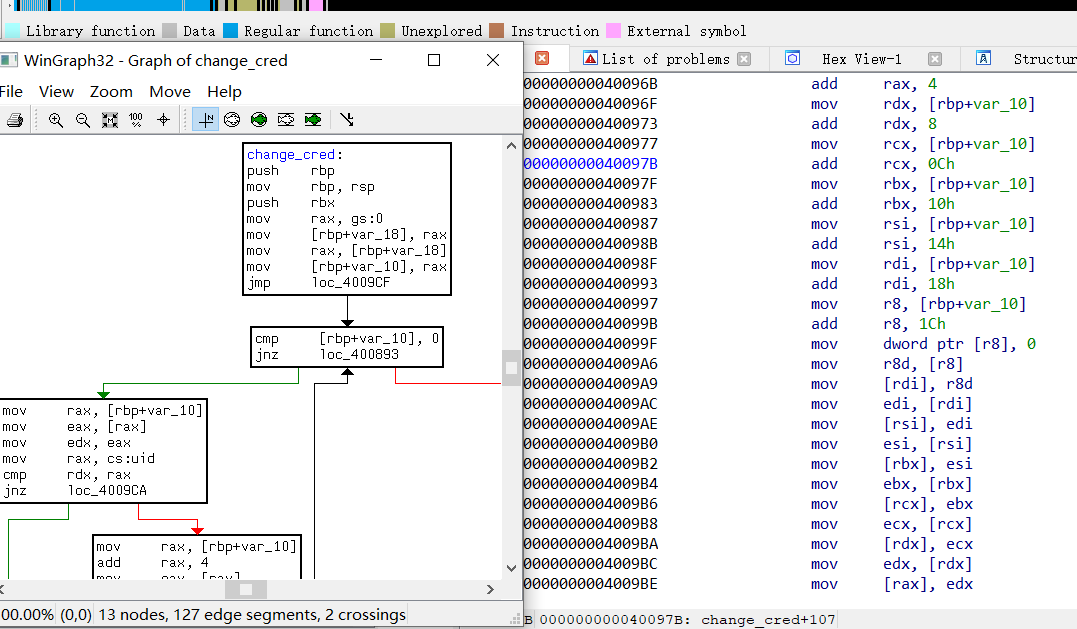
\includegraphics[width=0.75\textwidth]{figures/4.1}
	% \caption[这里的文字将会显示在 listoffigure 中]{这里的文字将会显示在正文中}
	\caption{IDA 反汇编 CFG 图}\label{fig:4.1}
\end{figure}


为确保扰动操作不影响原始程序逻辑,本文首先将反汇编得到的指令转换为一种自定义的中间表示(IR),该表示能记录每条指令的操作码、显式与隐式操作数、寄存器读写关系、以及影响到的标志位等静态语义信息。这种增强表示形式可有效辅助分析控制依赖与数据依赖关系,识别出可安全修改的指令区域。随后,本文实施三种语义保持的扰动技术:指令替换(Instruction Substitution)、指令重排序(Instruction Reordering) 和 寄存器重分配(Register Reallocation)。这三类方法分别从指令级别、顺序层级和寄存器使用层面引入扰动,旨在保持语义不变的前提下实现样本多样性和模型鲁棒性提升。

在变换过程中,所有修改操作均限制在已识别的、无控制依赖冲突的基本块内部,确保程序控制流图(CFG)保持稳定。如果某些变换操作(如指令顺序调整)导致代码地址偏移,本文会同步更新 ELF 文件中的相关重定位信息(如 .rela.text 段),以避免函数调用或跳转地址错误。整个扰动流程针对每个 ELF 文件独立执行,可自动生成多个等价但具有不同语法表现的扰动样本,用于训练或测试阶段的多样化增强,从而有效提升基于静态分析的恶意代码检测系统的鲁棒性。

(1) 指令替换(Instruction Substitution)

指令替换作为一种二进制代码扰动方法,旨在通过将原始指令替换为等效的指令来扰乱程序的结构,同时保持程序的功能不变。该方法不仅能改变代码的外观,还能增加静态分析和逆向工程的难度。以下是指令替换的具体细节:

等效指令替换在x86架构中,许多指令有多个等效形式,可以用不同的操作数或指令格式来实现相同的功能。例如:

add r/m32, r32 可以替换为 add r32, r/m32,这两者在操作数为寄存器时是等效的。

对于逻辑操作,test r/m8, r8 可以与 test r/m8, r/m8 等价。

一些算术指令也有多个等效形式,比如 sub r/m32, r32 可以用 neg r/m32 替换(减法可以通过取负来实现)。

操作数形式替换指令时,可以改变操作数的形式,而不影响最终的计算结果。例如,mov r32, r/m32 和 mov r/m32, r32 都是等效的操作,但通过改变源和目标操作数的顺序,能够改变指令的字节表示。

不同长度指令某些情况下,可以用长度相同但操作不同的指令替换原始指令,例如:

inc r32可以替换为 add r32, 1,二者功能相同,但指令长度和编码不同。

dec r32可以替换为 sub r32, 1,实现同样的效果,增加了代码的复杂性。

替换控制流指令 控制流指令(如跳转、条件跳转、调用等)也可以用等效的指令替换。例如:
jmp label 可以用 call label; pop 来替换,虽然实现了相同的跳转效果,但操作数和指令形式不同。

je(等于跳转)可以替换为 jne(不等于跳转),并通过适当调整标志位来维持功能一致性。

确保指令长度一致由于对于许多stripped二进制文件,增加指令长度可能会导致代码结构破坏,因此在替换过程中要保证每条替换的指令与原指令长度相同。可以通过选择长度一致的等效指令来实现这一点,避免扰乱程序的整体布局。

随机化替换的应用方式在替换指令时,可以根据一定的规则或随机选择等效指令来应用这些替换。替换不一定是对每条指令都应用,而是根据程序的特性和分析结果,选择性地对特定代码块进行替换。这种方法可以确保替换不会影响程序的控制流和逻辑结构,但同时会改变程序的外观,增加静态分析的难度。

通过以上方法,指令替换不仅保持程序功能的完整性,还有效增加了程序的混淆性,使得静态分析工具更难识别程序的真实意图,增加了逆向工程的复杂性。

(2)指令重排序(Instruction Reordering)

基本块内部指令重排(Intra Basic Block Reordering):在一个基本块(Basic Block)中,若两条或多条指令之间没有数据或控制依赖关系,那么它们的执行顺序就是可以互换的。由于基本块是线性执行的中间代码区域,并且编译器在生成机器码时只是选择了若干等效顺序之一,因此只要保证依赖关系不变,修改指令顺序不会影响程序的功能。

本文对目标二进制程序进行反汇编,提取所有基本块。对每个基本块进行依赖分析,识别每条指令的读(use)和写(def)寄存器集。通过检测读后写(RAW)、写后读(WAR)、写后写(WAW)等依赖类型,构建出指令间的有向无环图(DAG)。

之后,使用拓扑排序枚举该图的合法指令顺序,并从中随机选取一种新的顺序,替代原始顺序。这一方法不会引入新的指令或修改指令操作数,因此保持程序的功能完全不变。它可以扰乱基于指令顺序或特征码的静态分析和检测机制,有效提升样本的多样性。

\begin{figure}[hbt]
	\centering
	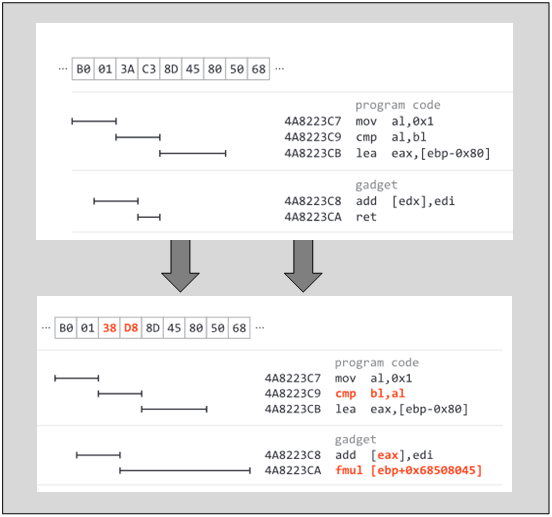
\includegraphics[width=0.75\textwidth]{figures/4.2}
	% \caption[这里的文字将会显示在 listoffigure 中]{这里的文字将会显示在正文中}
	\caption{指令替换示例图}\label{fig:4.2}
\end{figure}

寄存器保护代码重排(Reordering of Register Preservation Code):该方法基于函数调用时保存非易失性寄存器(callee-saved registers)所使用的push和pop指令的顺序是可变的,只要遵循“先进后出”的栈规则即可。即,函数在开头会使用若干push指令保存寄存器,函数结尾使用对应的pop恢复值。因为栈是倒序恢复的,所以只要保持pop顺序与push顺序相反,整个过程的语义就是等效的。

本文在函数的入口和出口识别出完整的寄存器保存/恢复代码段。对这些push和pop指令进行配对,确认其保护的是相同的寄存器,并追踪栈指针(ESP)的变化确保没有中间干扰。然后,对push序列进行重排,并将pop序列同步做相反的重排,确保恢复顺序正确。若push序列中夹杂有其他非保存性指令,也需进行依赖分析,保证重排不会打乱依赖顺序。这种方法对程序语义无影响,但能干扰基于特定pop序列模式的分析方法,提高静态分析、指令特征提取和样本分类的复杂度。

\begin{figure}[hbt]
	\centering
	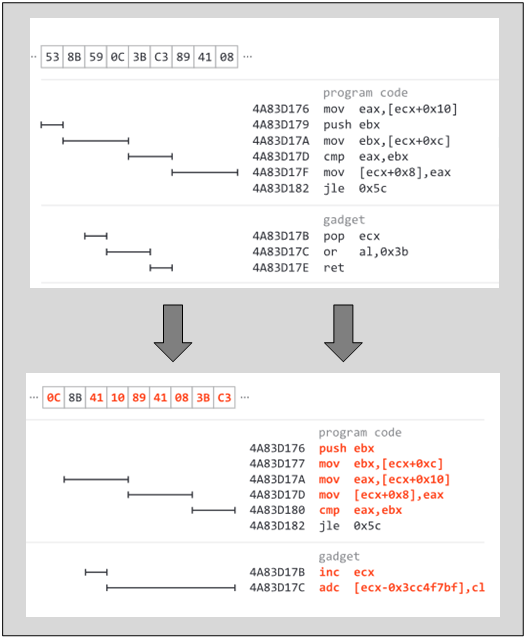
\includegraphics[width=0.75\textwidth]{figures/4.3}
	% \caption[这里的文字将会显示在 listoffigure 中]{这里的文字将会显示在正文中}
	\caption{指令重构排序示例图}\label{fig:4.3}
\end{figure}

\begin{figure}[hbt]
	\centering
	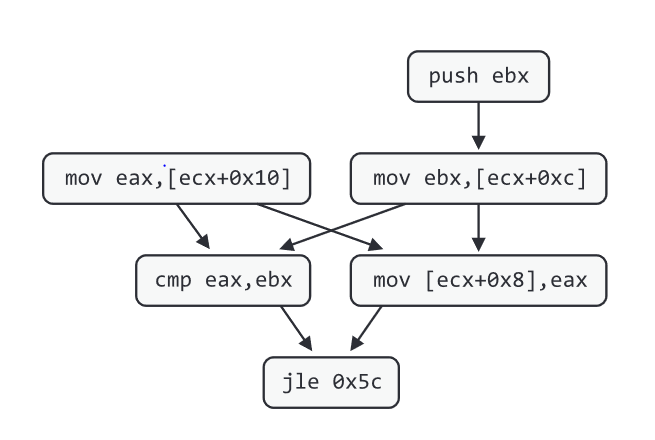
\includegraphics[width=0.75\textwidth]{figures/4.4}
	% \caption[这里的文字将会显示在 listoffigure 中]{这里的文字将会显示在正文中}
	\caption{重构的指令有序无环图}\label{fig:4.4}
\end{figure}

\begin{figure}[hbt]
	\centering
	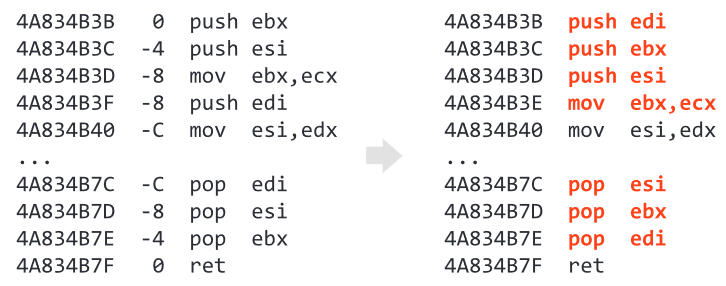
\includegraphics[width=0.75\textwidth]{figures/4.5}
	% \caption[这里的文字将会显示在 listoffigure 中]{这里的文字将会显示在正文中}
	\caption{寄存器保护代码重排序示例图}\label{fig:4.5}
\end{figure}

本文首先对二进制程序构建控制流图(CFG),并对每个基本块进行寄存器活跃性分析,获取每条指令的寄存器use(使用)与def(定义)集合。接着迭代计算每条指令的活跃输入集(in)与输出集(out),识别每个寄存器的活跃区域。在确保无冲突的前提下,随机选择两个不重叠活跃区的寄存器对,将其在汇编中的使用位置进行替换。指令修改时,通过变更ModR/M字节(必要时SIB字节)实现重映射,避免使用esp等特殊寄存器,并对隐式使用寄存器的指令进行过滤。为保证调用一致性,还需结合调用约定信息约束某些寄存器的使用。

这一方法不会引入新指令或修改操作数值,仅在机器码层面更换寄存器编号,因此程序行为保持完全一致。该技术能有效打乱静态分析工具基于寄存器使用模式或特征序列的识别策略,从而提升样本的对抗性与多样性。

\begin{figure}[hbt]
	\centering
	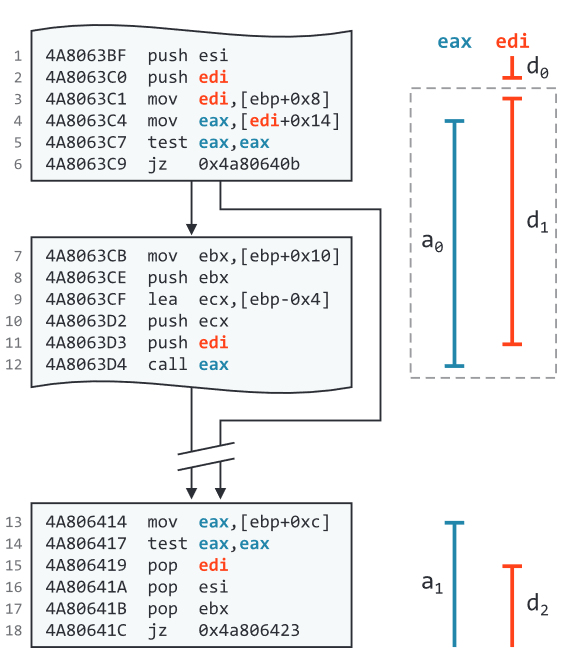
\includegraphics[width=0.75\textwidth]{figures/4.6}
	% \caption[这里的文字将会显示在 listoffigure 中]{这里的文字将会显示在正文中}
	\caption{寄存器重分配示例图}\label{fig:4.6}
\end{figure}

\subsection{动态行为扰动方法}

在恶意软件检测领域,动态分析技术是当前主流手段之一,尤其在处理未知样本或多态变种时具有明显优势。其基本原理是通过在受控执行环境(如沙箱、虚拟机、内存监控器)中运行目标程序,记录其在运行过程中所触发的系统调用、行为路径、内存修改、网络通信等信息,以此识别潜在的恶意行为。然而,这一技术在实际部署中往往存在时间资源受限的问题。为了兼顾效率与成本,动态分析系统通常仅为每个样本分配数秒到几十秒的执行时间窗口。对于某些攻击行为触发依赖于条件判断、用户交互的恶意样本而言,这一固定的分析时间窗显然存在被规避的可能性。

基于此观察,本文设计了一种动态扰动方法,核心思想是引入“时间延迟”机制,使恶意代码在样本启动后故意等待一段时间再执行核心逻辑,从而躲避沙箱的行为分析窗口。其主要实现方式是通过在程序入口点或关键路径中插入延迟逻辑(如 nanosleep系统调用),使恶意样本在运行初期不表现任何异常行为,从而骗过基于行为特征的检测系统。

具体而言,该方法在程序入口\_start 中插入一段系统调用延迟逻辑,构造一个 timespec结构体设置延迟时间(如60秒),并通过nanosleep系统调用实现挂起效果。在延迟期间,样本处于休眠状态,不触发任何系统调用,也不进行内存读写、网络通信等可疑操作。由于大多数沙箱系统会在执行时间到达后强制中止进程,此时还未触发的恶意行为链将完全无法被观测到。这样,恶意样本即使具有明显的破坏性,也可能因“未表现行为”而被误判为正常程序。

该策略可归类为一种“动态行为隐藏技术”,其本质在于对行为时间的扰动,从时间维度上对抗行为检测系统。这类技术的优势在于实现成本低、兼容性好且对原有逻辑无破坏性,能够与其他扰动策略(如控制流平坦化、代码插桩、系统调用替换)联合使用,从而形成更强的检测对抗能力。

值得注意的是,虽然该策略在现实场景中具有较强的隐蔽性,但其也可能被高级动态检测系统检测到。例如某些系统会使用加速执行技术(如时间跳跃模拟)、分析行为间歇性、或启用用户交互模拟等手段来破除延迟机制。因此,未来仍需结合其他对抗策略,共同提升样本的免杀能力和对抗鲁棒性。
\begin{algorithm}[htbp]
	\caption{使用可执行段填充空间进行 ELF 动态插入算法}
	\KwIn{目标 ELF 二进制文件路径 \texttt{input\_elf},载荷二进制代码路径 \texttt{code\_bin},输出 ELF 路径 \texttt{output\_elf}}
	\KwOut{一个已被感染的 ELF 文件,其中插入了载荷代码}
	Read the input ELF file \texttt{input\_elf} into memory \texttt{hdr}\;
	Read the payload binary code \texttt{code\_bin} into memory \texttt{code}\;
	Validate ELF magic number and ensure it is a 64-bit ELF\;
	Check if the ELF architecture is x86-64\;
	\ForEach{program header \texttt{phdr} in \texttt{hdr}}{
		\If{\texttt{phdr} is executable (has \texttt{PF\_X} flag)}{
			Find the last section \texttt{last\_sec} within \texttt{phdr}\;
			Compute the available padding size \texttt{pad\_size} after \texttt{last\_sec}\;
			\If{\texttt{pad\_size} $<$ size of \texttt{code} + size of jump}{
				Print error message and exit\;
			}
			Inject the payload \texttt{code} into the padding space\;
			Generate a jump instruction \texttt{jmp\_back} to the original entry point\;
			Inject \texttt{jmp\_back} after the \texttt{code}\;
			Modify the section header of \texttt{last\_sec} to extend its size\;
			Update the \texttt{phdr}'s file and memory size to include the injected code\;
			Update the ELF header's \texttt{e\_entry} to point to the start of the payload \texttt{code}\;
			\textbf{break}\;
		}
	}
	Write the modified ELF to \texttt{output\_elf}\;
	Set the file permission of \texttt{output\_elf} to executable\;
\end{algorithm}

基于时间延迟的动态扰动方法是一种有效的动态对抗技术,具有实现简单、效果明显、通用性强等优点,可作为恶意样本在强化学习训练与对抗生成中的关键扰动操作之一,具体实现如算法1所示。


算法1通过逐步操作,实现将载荷二进制代码动态插入到目标ELF可执行文件的可执行段填充空间中,保持原文件结构的同时实现控制流重定向。第1至2行将目标ELF文件与待插入的payload读入内存。第3至4行验证ELF文件的合法性,包括magic、是否为64位及是否为x86-64架构。第5至17行是注入的核心步骤:遍历每个程序头,第6行判断是否为可执行段(具有PF\_X标志),第7至8行定位该段的最后一个节并计算其后的空隙空间大小;若填充不足以插入payload与跳转指令,则退出(第9至10行)。第11至13行将载荷写入空隙并附加一段跳转回原始入口点的代码。随后,第14至15行扩展节和段的大小字段以覆盖新注入区域,确保在运行时被正确加载。第16行更新ELF头中的入口地址e\_entry为payload的起始位置,实现控制流重定向。完成注入后(第17行),退出循环以防止重复操作。最后,第18至19行将修改后的ELF写入输出文件并设置为可执行。整体流程在不破坏原有功能的前提下,实现了高隐蔽性和完整性兼容的动态插入操作。




\section{动态奖励函数策略优化(DRFOS)}

传统对抗样本生成方法多采用固定或静态的奖励函数,往往仅考虑单一的检测规避结果,例如是否成功逃避分类器或沙箱分析系统\cite{anderson2018learning}。然而,在实际应用场景中,恶意样本的行为表征、检测机制、资源限制(如沙箱分析时长)等因素均具备高度动态性。因此,本文设计一种自适应、阶段感知和行为敏感的动态奖励函数策略,对于提升对抗样本生成质量和鲁棒性具有重要意义。

本文提出一种动态奖励函数优化策略,结合多个维度的行为表现动态调整奖励函数,以提升样本的逃避能力、生成效率与混淆性。

在基于强化学习的对抗恶意样本生成框架中,奖励函数设计是智能体学习策略的核心驱动力。传统对抗样本生成方法多采用固定或静态的奖励函数,往往仅考虑单一的检测规避结果,例如是否成功逃避分类器或沙箱分析系统。然而,在实际应用场景中,恶意样本的行为表征、检测机制、资源限制(如沙箱分析时长)等因素均具备高度动态性。因此,设计一种自适应、阶段感知和行为敏感的动态奖励函数策略,对于提升对抗样本生成质量和鲁棒性具有重要意义。

\subsection{奖励函数设计动机}

强化学习智能体的行为策略直接受其奖励信号驱动。若奖励仅依据“是否逃避成功”这一单一信号,则智能体可能在初始训练阶段陷入稀疏奖励困境,导致训练效率低下,策略不稳定,甚至难以收敛。为解决该问题,本方法引入多源奖励信号融合机制,综合以下三类指标:

规避性得分(Evasion Score):反映样本是否成功规避沙箱或机器学习检测模型,是核心奖励来源;

扰动成本(Perturbation Cost):衡量修改对原始样本的干扰程度,用于抑制过度修改,保持样本可执行性与语义一致性;

行为混淆度(Behavior Confusion Degree):衡量样本行为与正常软件的相似度,鼓励智能体生成更具隐蔽性的扰动策略。

\subsection{奖励函数表达形式}

定义智能体在时刻 $t$ 执行扰动动作 $a_t$ 后的奖励 $R_t$ 为多项加权组合:
\begin{equation}
	R_t = \lambda_1 \cdot R_{\text{evasion}} + \lambda_2 \cdot R_{\text{confusion}} - \lambda_3 \cdot R_{\text{cost}}
\end{equation}

其中,$R_{\text{evasion}}$ 表示若样本成功绕过沙箱或分类器则给予正奖励,否则为 0;$R_{\text{confusion}}$ 表示根据行为序列(如系统调用图)与良性样本的相似度计算得分,例如使用 Jaccard 相似度或结构相似性;$R_{\text{cost}}$ 表示扰动的代价,可以根据扰动次数、修改字节数以及修改位置的敏感度等进行计算;$\lambda_1$、$\lambda_2$ 和 $\lambda_3$ 为动态可调的权重参数。

\section{基于LSTM的PPO时序模型结构}

本章提出的基于PPO(Proximal Policy Optimization)与 LSTM(Long Short-Term Memory)结合的强化学习模型主要由四个部分组成:LSTM时间特征编码层、策略网络(Actor)、价值网络(Critic)以及PPO优化器。训练过程中,首先由策略网络根据当前环境状态生成动作概率分布,同时价值网络对当前状态进行价值评估。为了能够有效建模动作序列中的时间依赖性,引入了LSTM模块,使得模型能够记忆过去的历史状态信息,捕获长期依赖特征,从而提升策略的稳定性与鲁棒性。最后,通过PPO优化器对策略进行迭代更新,保证训练过程中策略更新的稳定性与高效性。


\begin{algorithm}[htbp]
	\caption{基于强化学习的 ELF 对抗样本生成算法}
	\KwIn{原始 ELF 恶意样本集 $S$,最大迭代次数 $I$,预训练模型 $M$(PPO+LSTM),免杀行为表 \texttt{Action\_table},检测结果记录表 \texttt{Re}}
	\KwOut{免杀后的样本集 $S$}
	初始化智能体 agent 与环境 env\;
	agent $\leftarrow$ PPO\_LSTM.load($M$)\;
	$R_d \leftarrow 0$\;
	\ForEach{$s \in S$}{
		env.reset()\;
		tag $\leftarrow$ env.detect($s$)\;
		$S_t \leftarrow [\ ]$\;
		\For{$i \leftarrow 1$ \KwTo $9$}{
			$S_t \leftarrow S_t + \texttt{env.extractor}(s, i)$\;
		}
		\For{$j \leftarrow 1$ \KwTo $I$}{
			act $\leftarrow$ agent.predict($S_t$, $R_d$)\;
			\If{tag == benign}{
				\textbf{break}\;
			}
			$s \leftarrow \texttt{env.step}(s, \texttt{Action\_table}[act])$\;
			$S_t \leftarrow [\ ]$\;
			\For{$i \leftarrow 1$ \KwTo $9$}{
				$S_t \leftarrow S_t + \texttt{env.extractor}(s, i)$\;
			}
			tag $\leftarrow$ env.detect($s$)\;
			
			计算规避性得分:\texttt{Evasion\_Score} $\leftarrow$ score\_function($s$)\;
			
			计算行为混淆度:\texttt{Behavior\_Confusion\_Degree} $\leftarrow$ calculate\_confusion\_degree($s$)\;
			
			计算扰动成本:\texttt{Perturbation\_Cost} $\leftarrow$ calculate\_perturbation\_cost($s$, \texttt{Action\_table}[act])\;
			
			\If{tag == benign}{
				$R_d \leftarrow 10 \cdot \texttt{coefficient1} + \texttt{Behavior\_Confusion\_Degree} - \texttt{Perturbation\_Cost}$\;
				\textbf{break}\;
			}
			\Else{
				$R_d \leftarrow \texttt{Behavior\_Confusion\_Degree} - \texttt{Perturbation\_Cost}$\;
			}
		}
		\texttt{Re[$s$]} $\leftarrow$ tag\;
	}
\end{algorithm}

算法2描述了通过强化学习(PPO+LSTM)模型生成ELF格式恶意样本的免杀对抗样本。第1至2行初始化智能体和环境,加载预训练的PPO+LSTM模型。第3行初始化奖励信号$R_d$为0。第4至6行遍历原始恶意样本集S并重置环境,检测样本的标签。第7至9行提取环境中的特征,并存储在状态$S_t$中。第10至26行是主要的扰动步骤:智能体根据当前状态和奖励预测执行动作。第11至12行通过智能体的预测生成扰动动作,并根据样本标签(恶意或良性)决定是否继续执行。第13至15行,执行动作后更新样本并提取新的环境特征。第16至18行,计算新的奖励值,综合考虑规避性得分、行为混淆度和扰动成本。第19至24行根据检测结果和扰动成本动态计算奖励值,如果样本成功规避检测则给予较高的奖励,否则计算扰动成本并适当降低奖励。第27行更新样本的标签并记录在检测结果表Re中。整个流程通过多源奖励信号的融合与动态调整,逐步优化智能体的策略,以生成能够有效绕过检测并保持样本可执行性的对抗样本。

\subsection{LSTM时间特征编码层}

在传统强化学习中,策略与价值估计往往只基于当前状态单步决策,忽略了历史决策之间的时间关联性,容易导致短视行为。

为此,本模型在输入端引入了LSTM(长短期记忆网络),通过门控机制捕获长期依赖,增强决策的时序连贯性。

LSTM单元内部操作公式如下:

输入门(控制当前输入信息的流入):
\begin{equation}
i_t = \sigma(W_i x_t + U_i h_{t-1} + b_i)
\end{equation}

遗忘门(控制上一个记忆单元的保留程度):
\begin{equation}
f_t = \sigma(W_f x_t + U_f h_{t-1} + b_f)
\end{equation}

单元状态更新(生成新的记忆内容):
\begin{equation}
\tilde{c}_t = \tanh(W_c x_t + U_c h_{t-1} + b_c)
\end{equation}

单元状态(记忆细胞)更新:
\begin{equation}
c_t = f_t \odot c_{t-1} + i_t \odot \tilde{c}_t
\end{equation}

输出门(控制隐藏状态输出):
\begin{equation}
o_t = \sigma(W_o x_t + U_o h_{t-1} + b_o)
\end{equation}

隐藏状态更新(作为下一步输出):
\begin{equation}
h_t = o_t \odot \tanh(c_t)
\end{equation}

其中,$\sigma$ 为 Sigmoid 激活函数,$\odot$ 表示 Hadamard 乘积(元素乘),
$x_t$ 是当前时刻的输入状态,$h_{t-1}$ 和 $c_{t-1}$ 分别是上一时刻的隐藏状态与单元状态。

通过以上机制,LSTM 能有效捕捉输入状态序列中的长期依赖特征,使策略网络与价值网络
具有更强的历史建模能力。

\subsection{策略网络(Actor)}

策略网络负责从环境中接收到的状态信息中,输出当前动作的概率分布。为了增强策略对于历史信息的感知能力,策略网络在输入端接入了LSTM层,LSTM能够在一定程度上记忆先前状态的隐藏信息,从而使得输出的策略不仅依赖当前时刻的观测,还综合考虑了历史观测序列的特征。
策略网络的目标是根据当前的隐藏状态 ,输出每个动作的概率分布 。
具体过程如下:

\begin{enumerate} [label=\arabic*)] 

\item LSTM编码后的隐藏状态  作为输入;

\item 经过多层感知机(MLP)映射至动作空间;

\item 通过 Softmax 函数输出动作分布:
\begin{equation}
\pi_{\theta}(a_t | s_t) = Softmax(W_p h_t + b_p)
\tag{4.8}
\end{equation}
其中,$W_p$、$b_p$ 为策略网络的权重与偏置参数,$\theta$ 表示策略网络的参数集合;

\item 依据动作概率分布进行采样,生成动作 $a_t$:
\begin{equation}
a_t \sim \pi_\theta(a_t | s_t)
\end{equation}

\end{enumerate}

\subsection{价值网络(Critic)}

价值网络负责对当前状态的价值进行估计,即预测从当前状态出发,在未来遵循当前策略所能获得的期望回报。与策略网络类似,价值网络同样引入了LSTM编码层,以捕获状态序列中的时间关联性,提升价值估计的准确性和稳定性。

价值网络旨在估计当前状态  的状态价值函数 ,即从状态  出发,在未来遵循当前策略  所能获得的期望总回报。与策略网络结构类似,价值网络也基于LSTM编码后的隐藏状态 ,经MLP输出一个实数值:

状态价值估计:
\begin{equation}
V_{\phi}(s_t) = W_v h_t + b_v
\end{equation}

其中,$W_v$ 和 $b_v$ 分别为价值网络的权重与偏置参数,${\phi}$为价值网络参数集合。

\subsection{策略优化器}

PPO 引入了剪切(Clipped)目标函数,在更新策略时,限制新旧策略之间的变动范围,从而提高训练的稳定性。

首先定义概率比率 \(r_t(\theta)\):
\begin{equation}
	r_t(\theta) = \frac{\pi_{\theta}(a_t | s_t)}{\pi_{\theta_{\text{old}}}(a_t | s_t)} \tag{4.11}
\end{equation}

其中,\(\pi_{\theta_{\text{old}}}\) 表示上一次更新前的策略参数。

优势函数(Advantage)定义为:
\begin{equation}
	A_t = \delta_t = r_t + \gamma V(s_{t+1}) - V(s_t) \tag{4.12}
\end{equation}

其中,\(r_t\) 为即时奖励,\(\gamma\) 为折扣因子。

PPO 的最终优化目标为:
\begin{equation}
	L^{\text{CLIP}}(\theta) = \mathbb{E}_t \left[ \min \left( r_t(\theta) A_t, \ \text{clip}\big(r_t(\theta), 1-\epsilon, 1+\epsilon\big) A_t \right) \right] \tag{4.13}
\end{equation}

当 \(r_t(\theta)\) 处于 \((1-\epsilon, 1+\epsilon)\) 区间内时,直接使用真实比率乘以优势函数;当超出该区间时,使用裁剪后的比率,防止策略更新幅度过大。

价值函数损失(均方误差)为:
\begin{equation}
	L^{\text{VF}}(\varphi) = \mathbb{E}_t \left[ \left(V_{\varphi}(s_t) - R_t\right)^2 \right] \tag{4.14}
\end{equation}

其中,\(R_t\) 是累积回报(真实价值目标)。

最终的整体损失函数(综合考虑策略损失、价值损失和熵正则化)为:
\begin{equation}
	L(\theta, \varphi) = L^{\text{CLIP}}(\theta) - c_1 L^{\text{VF}}(\varphi) + c_2 S[\pi_{\theta}] \tag{4.15}
\end{equation}

其中,\(S[\pi_{\theta}]\) 为策略熵,用以鼓励探索;\(c_1\) 和 \(c_2\) 为损失权重系数。

\section{本章小结}

本章介绍了基于强化学习的恶意软件对抗样本生成技术,重点阐述了如何利用强化学习与多种扰动方法相结合,生成能够有效规避恶意软件检测模型的对抗样本。介绍了利用强化学习优化扰动策略的方式,使生成的恶意软件样本在保证隐蔽性的同时,能够有效规避多个检测模型的识别。接着介绍了本章所提出的奖励函数优化方案,以及详细介绍了提出的基于LSTM的PPO时序模型的具体实现。




